Graph databases are a type of NoSQL database designed to store, manage, and query data that is highly interconnected. Unlike traditional relational databases, which organize data in tables, graph databases represent data as a graph composed of nodes, edges, and properties.

\textbf{Nodes:} These represent entities or objects in the database, such as people, places, or items.

\textbf{Edges:} These define relationships between nodes. For instance, an edge can represent a ``friendship'' relationship between two nodes representing people.

\textbf{Properties:} Both nodes and edges can have properties, which are key-value pairs that provide additional information about the nodes and edges. For example, a node representing a person might have properties like ``name'' and ``age,'' while an edge representing a friendship might have a property ``since'' indicating when the friendship started.

Graph databases are particularly powerful for applications that involve complex relationships and dynamic schemas. Examples include social networks, recommendation systems, and fraud detection systems.

\subsection{Types of Graph Databases}

Graph databases can be implemented using different underlying concepts for representing data. The two most common such concepts in graph databases are RDF (Resource Description Framework) and LPG (Labeled Property Graphs).\footnote{Angels, R. (2012) A Comparison of Current Graph Database Models. 2012 IEEE 28th International Conference on Data Engineering Workshops}
Both RDF and LPG has a graph as it's underlying concept but differs in how the data is stored in the graph. RDF use a triple of a subject, predicate and object, all encapsulated in URLs as their underlying data structure. The subject is the resource that is being described, the predicate is a property or characteristics of the subject and the object is the value of the property. Because all data is encapsulated in URLs RDF is useful when the represented data is already in the form of an URL. Meaning that when the data is in the web an RDF database could be useful. The subject, the predicate and the value does not have attributes or associated key value pairs. In order to add information about the relationships the subject in a triple of subject, predicate and object, has to be a triple itself. 

In LPG the data is represented in the nodes and the edges between the nodes. The entities, or nouns, are represented as nodes and the relationships between the entities are represented in the edges. Both the nodes and the edges can be labeled with attributes about the entity or the relationship. Attributes are specified in a key value structure. An attributes about a relationship between two entities is therefore specified in the relation itself. Neo4j is a graph database that has LPG as it's underlying concept.

\subsection{Key Features of Graph Databases}

\textbf{1. Schema-Free:} Graph databases are typically schema-free, meaning the data model can evolve without the need for predefined schemas. This flexibility allows for easier adjustments and scalability as data and relationships grow.

\textbf{2. Efficient Relationship Handling:} Graph databases excel at managing and querying complex relationships. Traversing relationships in a graph database is more efficient than performing multiple joins in a relational database.

\textbf{3. Query Languages:} Graph databases use specialized query languages designed for graph traversal and pattern matching. The most notable query language for graph databases is Cypher, used by Neo4j. Cypher provides a syntax that is easy to learn and allows for expressive and efficient graph queries.



% Cypher and Neo4j will be used as examples in the comparison with relational databases. Some knowledge of SQL is expected to understand the concepts discussed in this paper.

% % tables vs graphs, show an image of a table and a graph
% % add image from assets filder
% \begin{figure}[ht]
%     \centering
%     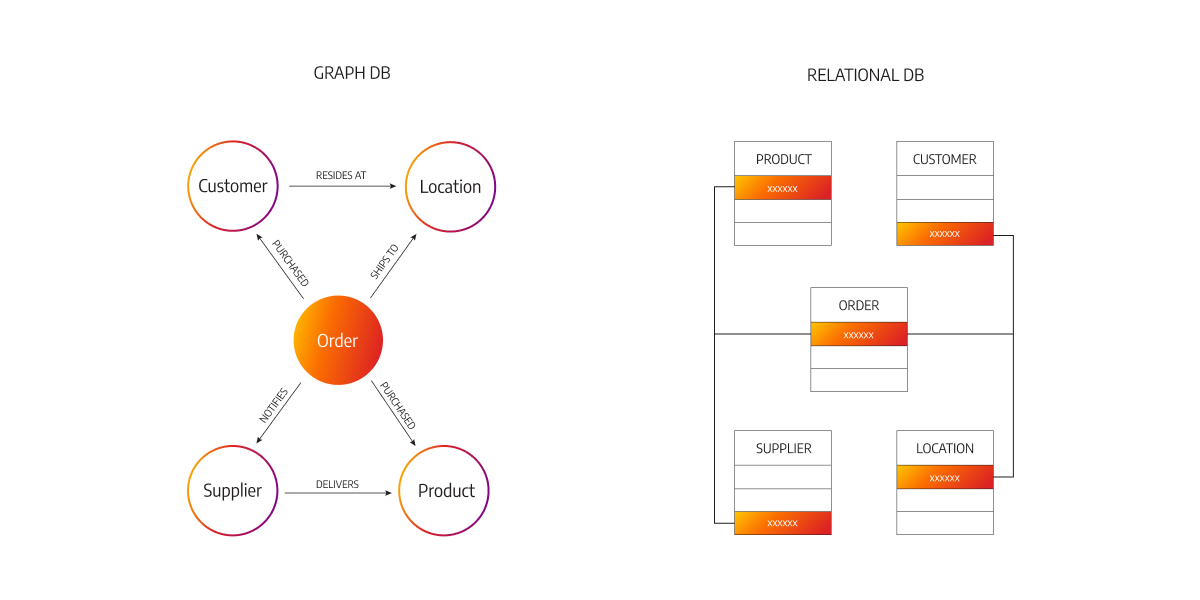
\includegraphics[width=0.7\textwidth]{assets/memgraph-graph-database-vs-relational-database.png}
%     \caption{Comparison of graph databases vs. relational databases.\protect\footnote{Image source: Memgraph, \url{https://memgraph.com/blog/graph-database-vs-relational-database}}}
%     \label{fig:graph_vs_table}
% \end{figure}
% In Figure \ref{fig:graph_vs_table}, we see a comparison of graph databases and relational databases. The graph database on the left shows a graph schema, while the relational database on the right shows a relational schema. The graph schema shows nodes and relationships between nodes, while the relational schema shows tables and relationships between tables. 

% \begin{figure}[ht]
%     \centering
%     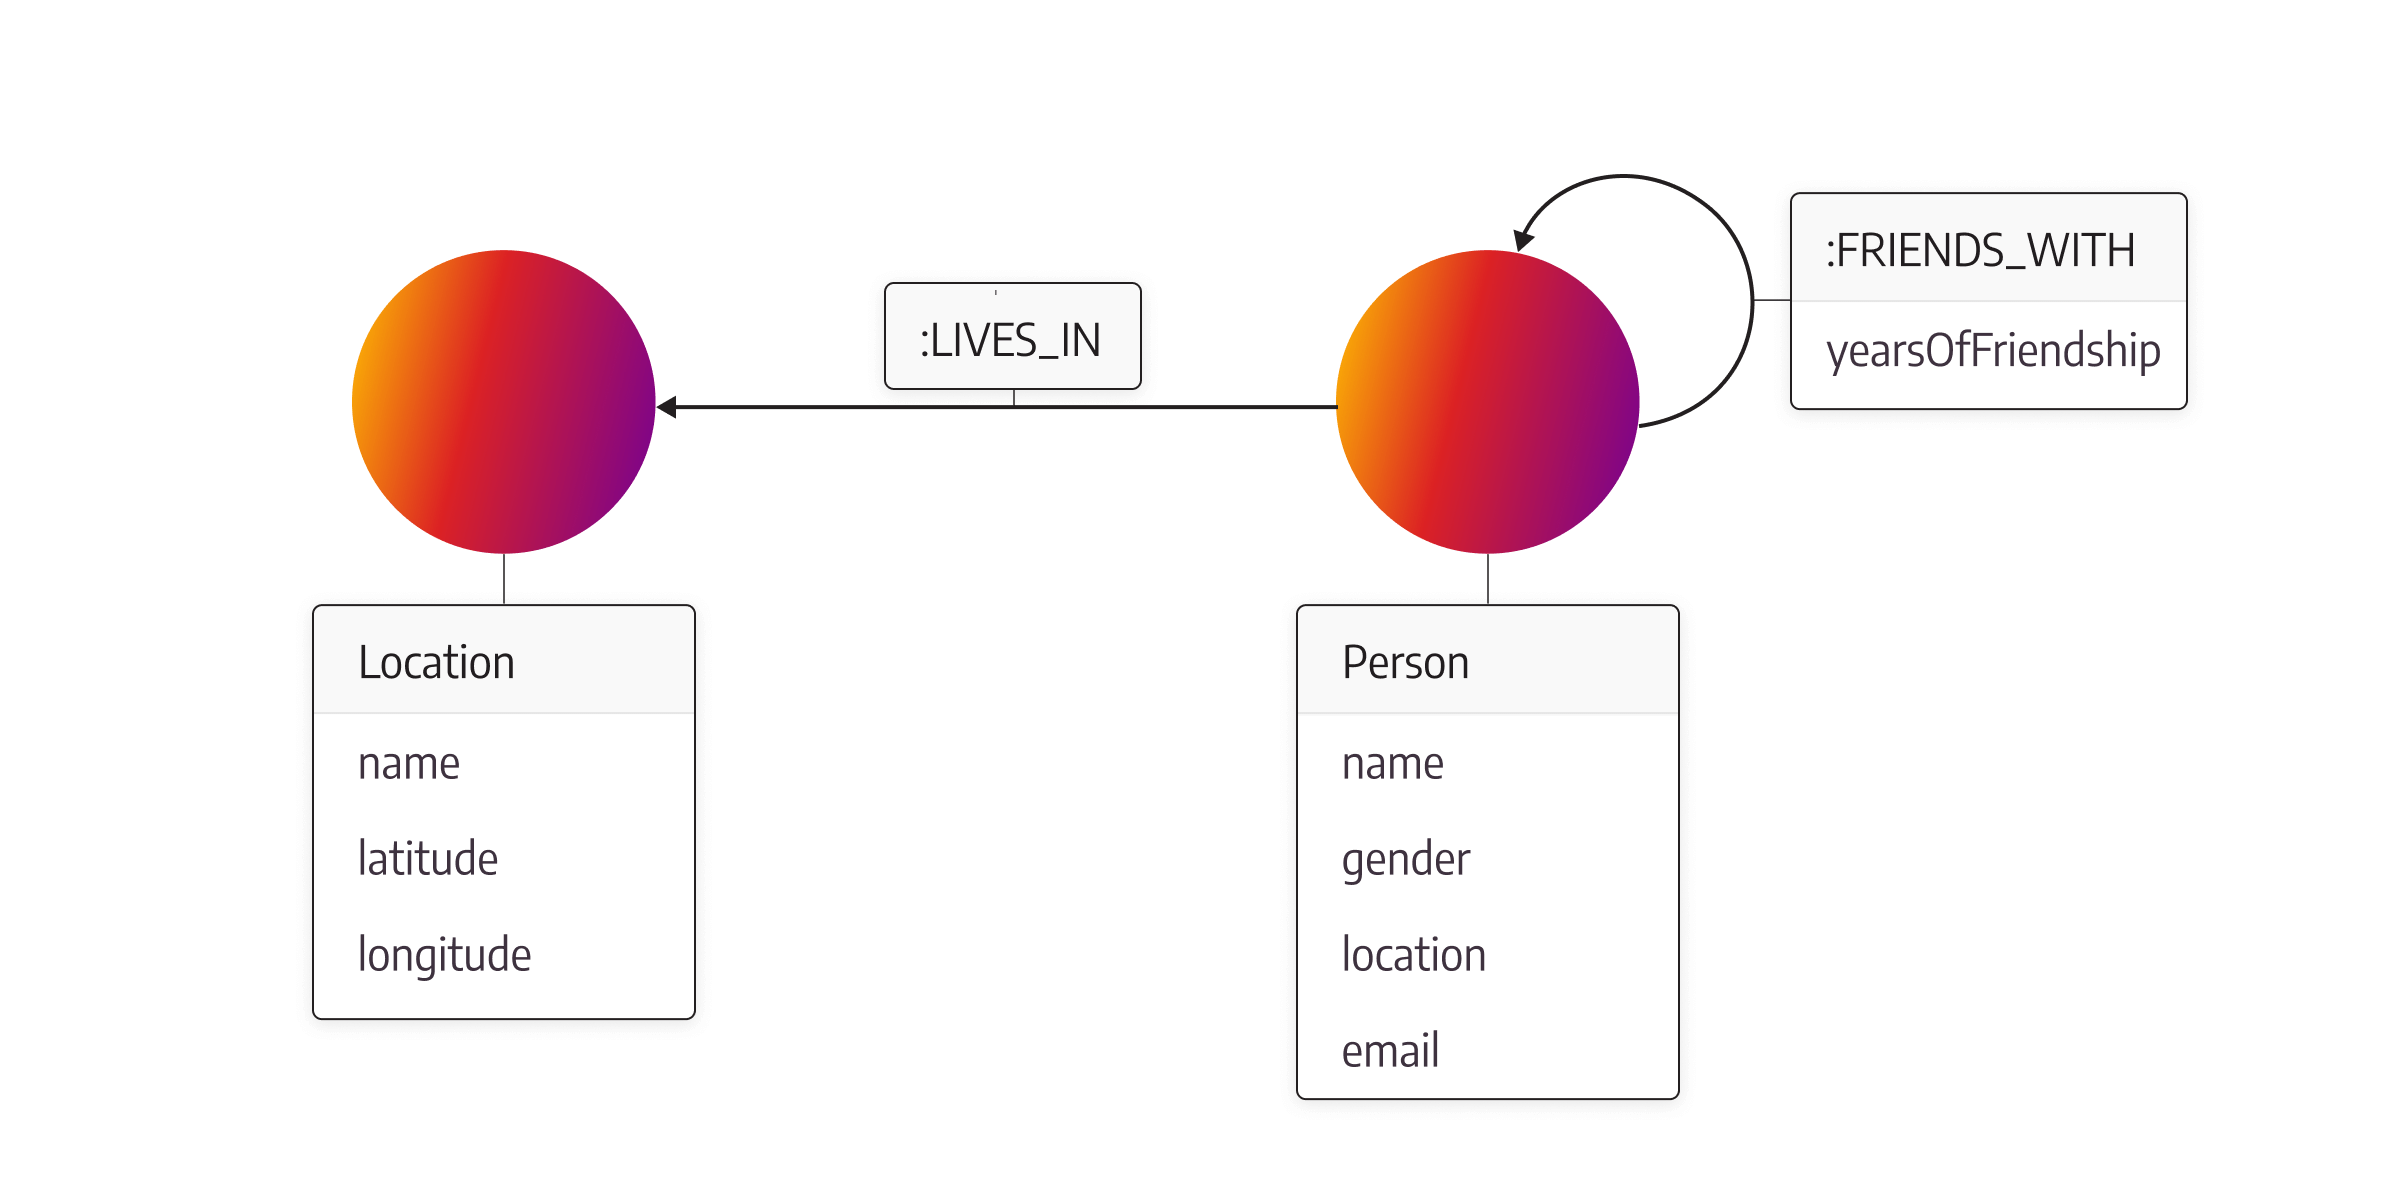
\includegraphics[width=0.7\textwidth]{assets/memgraph-graph-schema.png}
%     \caption{Graph Schema.\protect\footnote{Image source: Memgraph, \url{https://memgraph.com/blog/graph-database-vs-relational-database}}}
%     \label{fig:graph_schema}
% \end{figure}
% In Figure \ref{fig:graph_schema}, we see a graph schema. The graph schema shows nodes and relationships between nodes. The nodes represent entities, while the relationships represent the connections between entities. 

% \begin{figure}[ht]
%     \centering
%     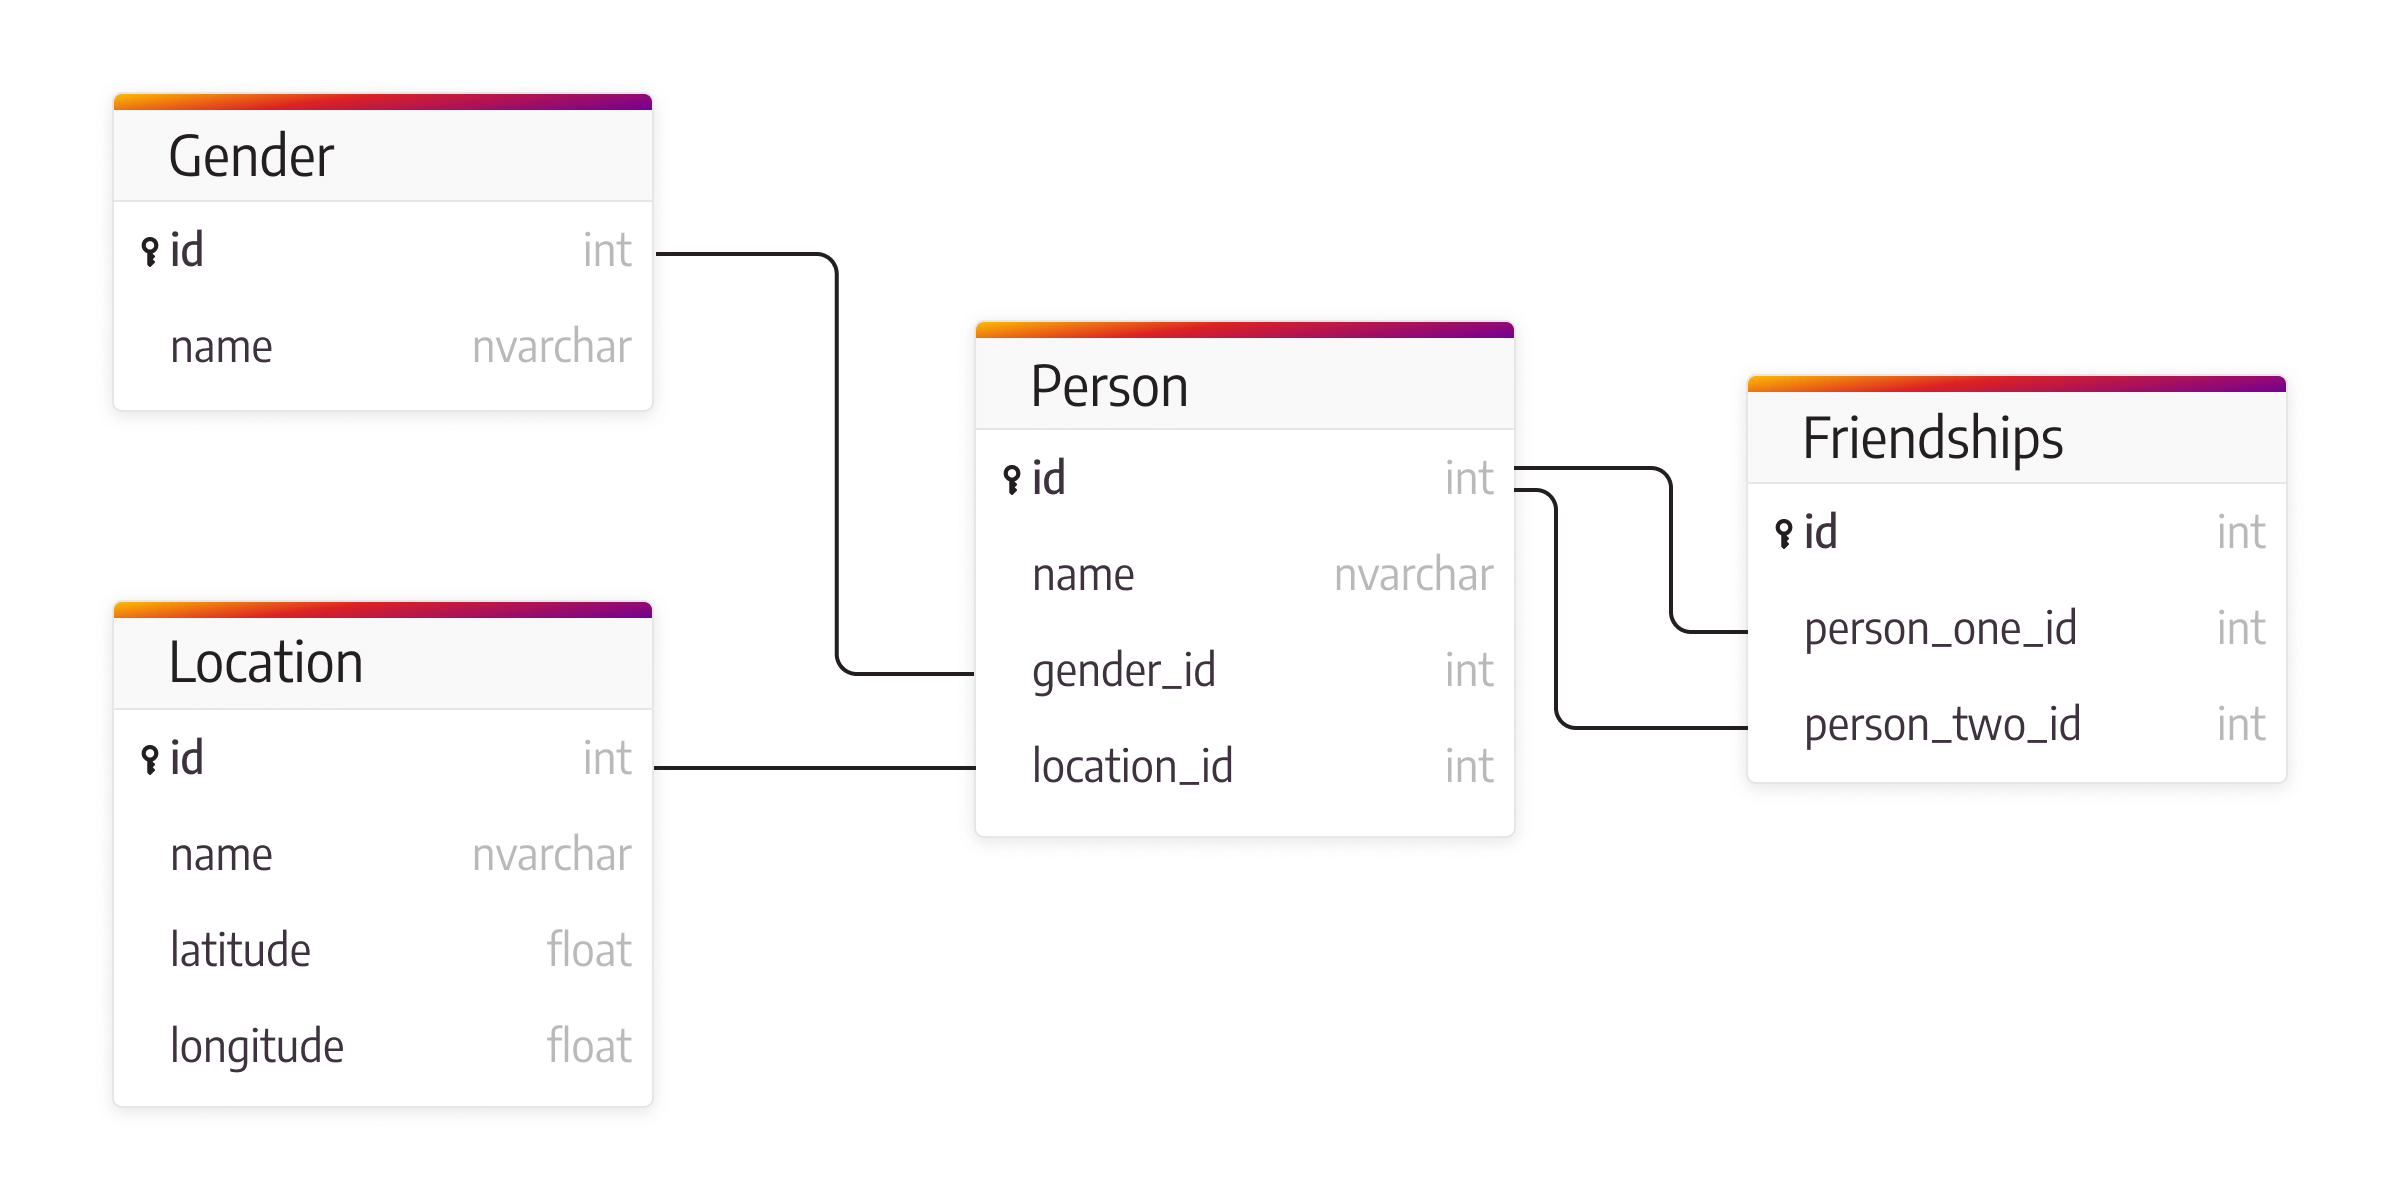
\includegraphics[width=0.7\textwidth]{assets/memgraph-relational-schema.png}
%     \caption{Relational Schema.\protect\footnote{Image source: Memgraph, \url{https://memgraph.com/blog/graph-database-vs-relational-database}}}
%     \label{fig:relational_schema}
% \end{figure}
% In Figure \ref{fig:relational_schema}, we see a relational schema. The relational schema shows tables and relationships between tables. The tables represent entities, while the relationships represent the connections between entities.